\chapter{Metadata Visualization}
\graphicspath{{figs/03-visualization/}}
\label{chapter:metadata-visualization}

Among the presented tools in chapter \ref{chapter:background}, MONTRA was our go-to mainly because of its data source-centric approach.
Also, no real data is shown here, only metadata is handled within the platform, however, it still allows to impose access permissions at several levels.

This chapter will be detailed the key concepts of the MONTRA framework and its internal data model.
After this, there will be presented a refactoring process that was done to the platform, with its improvements and flaws fixed.

\section{MONTRA}

%\begin{itemize}
%    \item O que é o montra e o seu estado atual
%    \item explicar de maneira mais aprefundada a paltaforma, realçando partes que devem ser alteradas ou que não estão corretas
%\end{itemize}

Originally, the MONTRA framework was developed by the Bioinformatics team of the Institute of Electronics and Informatics Engineering of Aveiro associated with the \gls{emif} project with the goal to develop a common patient health information framework with emphasis on the research topics of Obesity and its metabolic complications and Markers for the development of Alzheimer's disease and other dementias.
The code is publicly available on github\footnote{https://github.com/bioinformatics-ua/montra}, whereby Django 1.4, a high-level Python Web framework\cite{django}, was used as a framework to develop the entire system.
This framework allows to develop complete web applications, in a faster and easier way.
It contains a model layer that allows specifying database tables through python classes called models, following a \gls{orm} approach, allowing to perform database queries through python code instead of \gls{sql} queries.
Django can then check if there are new models or if existing ones have changed. Such changes are then expressed through database migration files which will apply them to the database tables.
Next, the developer can set custom URL patterns so specific requests are handled by a specific function of the view layer, where the business logic will be implemented.
Finally, Django contains a template layer that allows building dynamic \gls{html} pages without requiring to have a separate javascript framework to do such.
The developer builds the main static structure of the page and then uses a special syntax that describes how Django should display the data received from the view layer.
Django also has an import form feature that allows to easily create a set of pages that allow performing the usual \gls{crud} operation over the database model.

MONTRA's development started at the beginning of 2013 and ended in the middle of 2018.
After this date, at the end of 2018, the framework started being used by the \gls{ehden} project, to develop a portal to allow discovery and analysis of health data of a federated network of data sources standardized to the \gls{omop} common data model in Europe.
Currently, the project is being developed in a private repository but has intentions to make it public after the code base is more robust and well documented.

\subsection{Communities}

In the first versions of the framework, MONTRA allowed only one level of organization related to data sources, in which they could only be separated according to their skeleton that describe their original data, which will be more detailed in the next subsection.
Newer versions created the concept of a Community.
This allows having multiple networks of data sources on the same portal, where originally the only option was to have different installations of the framework.

These communities can be created in several ways:

\begin{enumerate}
    \item the admin can create it through Django's admin console
    \item a user can request a community to be created through a form and then the admin will receive an admin with such request
    \item the MONTRA installation can be deployed in a single community mode where only one community exists, which is created on the first setup, giving the idea that there is no community concept on the platform
\end{enumerate}

They also can have different access levels:

\begin{itemize}
    \item Open: Does not require membership. Any user can access the data sources of this community
    \item Public: Does not require a membership however, the user needs to accept a set of terms and conditions before being able to access the data sources
    \item Moderated: A user has to request the community managers for approval
    \item Invitation: Users can only access and see the community by invite and subsequent approval
\end{itemize}

\subsection*{Plugins}
The concept of Community also allows customization at that level, affecting only sections within that given community.
One example of such customization is plugins, a way to extend the functionalities of the framework without having to deal with the base code.
These plugins can either be full web applications, with different functionalities, that are linked to MONTRA through the community navigation menu or extensions that provide extra data services such as a dashboard about the data of a data source.

\subsection{Questionnaires}

%\begin{itemize}
%    \item questions
%    \item tipo de questoes
%\end{itemize}

As the data from different data sources is highly heterogeneous, MONTRA ensures that the data inserted within a given community follow a common structure.
This structure is called a skeleton, which is represented in a form of a questionnaire with a set of questions, which can then be grouped in sections called Question Sets.
It represents a set of metadata that betters describes the original data of data sources that need to remain private.
The skeleton schema can easily be defined through a spreadsheet, which will be more detailed on subsection \ref{subsection:excel}.

Next is presented the available question types which can be used to build a questionnaire for a community

\begin{longtable}[c]{|c|c|}
\hline
\textbf{Type}             & \textbf{Description}                                        \\ \hline
\endhead
choice                    & single choice (radio box)                                   \\ \hline
choice-freeform           & single choice with an open text fields                      \\ \hline
choice-multiple           & multiple choice (checkbox)                                  \\ \hline
choice-multiple-freeform  & multiple choice with and open text fields                   \\ \hline
choice-tabular            & creates a table with single, multiple choices or text by row      \\ \hline
choice-yesno              & single choice with yea and no choices                       \\ \hline
choice-yesnodontknow      & single choice with yes, no and don't know choices           \\ \hline
comment                   & used to separate groups of questions                        \\ \hline
custom                    & mirrors another question by its                             \\ \hline
datepicker                & field with date picker widget                               \\ \hline
email                     & text input with email validation                            \\ \hline
location                  & set of select elements to choose                            \\ \hline
numeric                   & numeric input                                               \\ \hline
open                      & text field with no validation                               \\ \hline
open-button               & text input with backend validation                          \\ \hline
open-location             & text input with autocomplete sugestions                     \\ \hline
open-multiple             & allows to record an history of a value overtime             \\ \hline
open-multiple-composition & allows to record an history of several values overtime              \\ \hline
open-textfield            & same as open but a textarea html tag is used                \\ \hline
open-upload-image         & image upload                                                \\ \hline
open-validated            & text input with a regex validation                          \\ \hline
publication               & a custom widget that allows to attach a set of publications \\ \hline
range                     & allows to define a range of numeric values                  \\ \hline
sameas                    & mirrors another question by its number                      \\ \hline
timeperiod                & numeric input + select to choose numeric unit               \\ \hline
url                       & text input with url validation                              \\ \hline
\caption{All available question types that can be used to build a questionnaire}
\label{tab:my-table}\\
\end{longtable}

\subsection{Fingerprints}

%\begin{itemize}
%    \item Views
%    \item validação feita toda do lado do cliente, existindo a possiblidade de ataques xss
%    \item a validação builtin do django não está a ser usada
%\end{itemize}

A fingerprint is a name given to the set of answers to the questions of a questionnaire.
In other words, it is the metadata that betters describes the original data of the associated data source.
Data owners can start to answer the questions to build the profile of their data sources once there are communities on the platform and, these have at least a questionnaire associated.

\begin{figure}[h]
    \center
    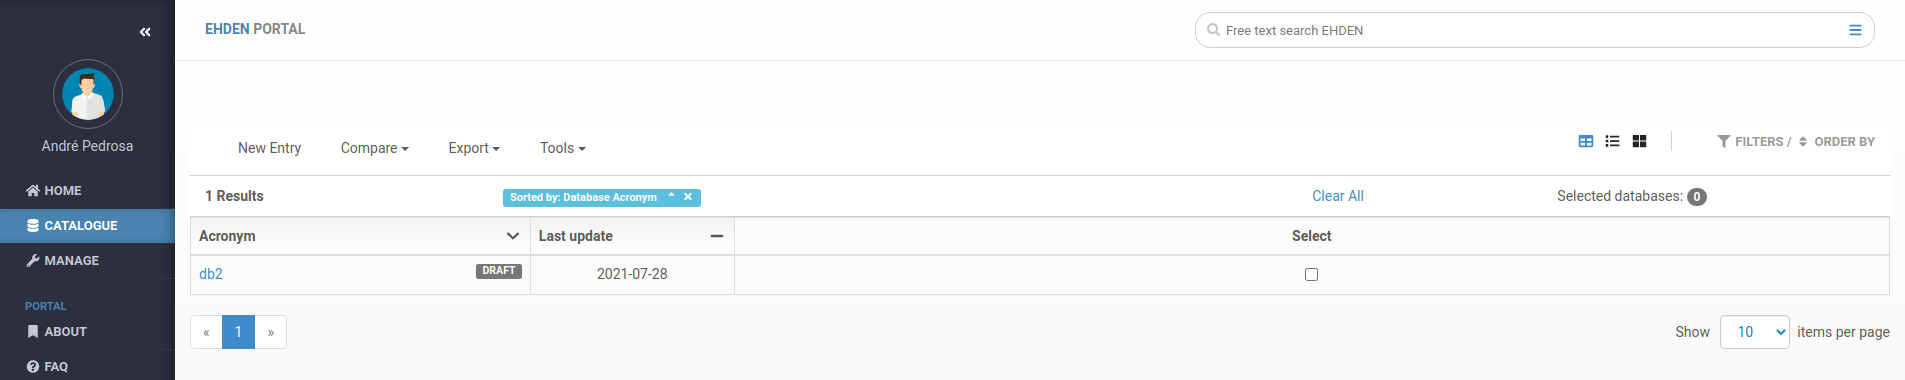
\includegraphics[width=\textwidth]{listings}
    \caption{The user interface displayed after selecting a community, which shows the list of the fingerprints of the chosen community}
    \label{fig:listings}
\end{figure}

On the list presented in figure \ref{fig:listings}, we can notice that the only fingerprint present is marked as draft.
This is a state of the fingerprint which prevents from non-ready or non-approved fingerprints won't show to the regular community users.
With this, for such users the list shows above would be empty.
Fingerprints can be published depending on the chosen settings for the community.
After the data source owners request to publish a fingerprint the framework allows to either automatically accept or require a community manger to accept it.

\subsection*{Views}

In figure \ref{fig:fingerprint-new} it is presented the user interface where a data owner can answer the questions of a questionnaire.
Each question of the questionnaire is placed under a container that can be collapsed, as is shown for question \textit{Instituition name}.
However, if multiple questions are grouped, the collapsable container will affect all questions of the group.
Besides the input widget where the data owner can insert its answers, the user also has some additional control buttons:

\begin{enumerate}
    \item Allows to Hide or Show Questions that have been answered or that are empty. Besides being an interesting feature is important to note that on the last version it does not work, as clicking on the presented options will result in no visual effect
    \item Allows to collapse or expand all questions or question groups containers
    \item Allows the data owners to set permissions at the question set level 
        \begin{itemize}
            \item Visibility: Let plugins have access to answers data
            \item Allow printing: On the fingerprints list page, showed in figure \ref{fig:listings}, there is a dropdown with tools, being the only one the "Print" tool (\ref{fig:listings-tools}). However, this feature is not correctly implemented since it calls the browser's built-int printing function on the fingerprint list page, so no actual fingerprint data will be printed. This permission ends up being useless. Additionally, if a user calls the browser's print function (e.g. hitting Ctrl+P) when viewing the data of a fingerprint, the platform will not block the action.
                \begin{figure}[h]
                    \center
                    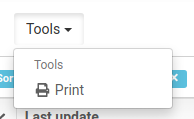
\includegraphics[width=.2\linewidth]{listings-tools}
                    \caption{Available tools on the fingerprint selection}
                    \label{fig:listings-tools}
                \end{figure}
            \item Allow indexing: If the data owner allows indexing of the answers, which will allow for other users to find fingerprints based on the answers to a question of this specific question set.
            \item Allow exporting: If the answers to this question set can be included on the export file of a fingerprint.
        \end{itemize}
    \item Enable navigation along the question sets of the current questionnaire
    \item Permits to save or cancel all the changes made to the current question set
\end{enumerate}

\begin{figure}[h]
    \center
    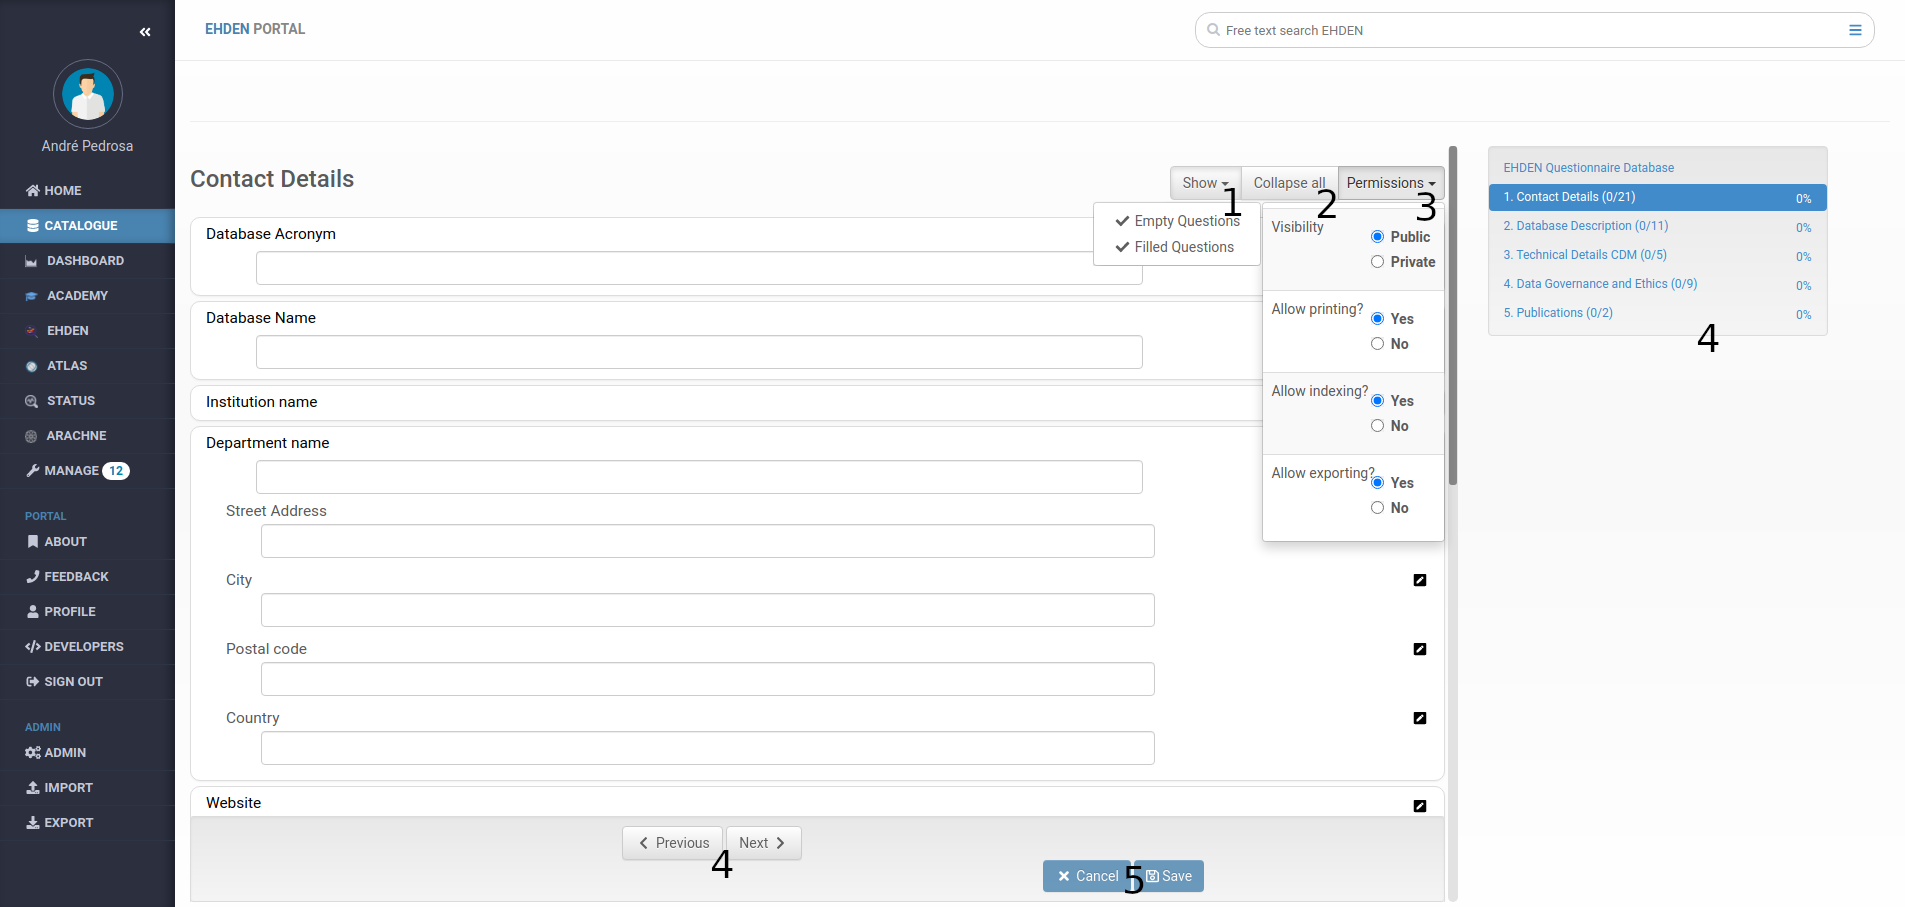
\includegraphics[width=\textwidth]{fingerprint-new}
    \caption{User interface to create a fingerprint}
    \label{fig:fingerprint-new}
\end{figure}

Once the fingerprint is filled and published, a regular user can consult the metadata, which will be displayed by default in detailed vie. Similar to the create view, it is presented with some control buttons:

\begin{enumerate}
    \item Database level plugins associated with this community
    \item Statistics of this fingerprint
        \begin{itemize}
            \item Progress bar + Filled: How many questions of the questionnaire were answered
            \item Hits: Number of times this fingerprint showed up on search queries
            \item Unique Views: Number of users that visited this fingerprint
        \end{itemize}
    \item Question set controls
        \begin{itemize}
            \item Summary: Allows to switch to the summary view (Figure \ref{fig:fingerprint-show-summary})
            \item Collapse \& Show: The same role as mentioned for the create view
        \end{itemize}
    \item Fingerprint control buttons
        \begin{itemize}
            \item Subscribe: Receive notifications whenever changes are made to the fingerprint answers
            \item Manage: Several fingerprint operations
                \begin{itemize}
                    \item Edit: Enter the edit mode
                    \item Share: Allows to add other users as owners of the fingerprint and also to create links that enable anonymous users to consult the fingerprint
                    \item Export: Different forms of export. CSV, PDF, and MONTRA format to import on other installations of the MONTRA framework
                    \item Delete: Remove the fingerprint from the community
                \end{itemize}
        \end{itemize}
\end{enumerate}

\begin{figure}[h]
    \center
    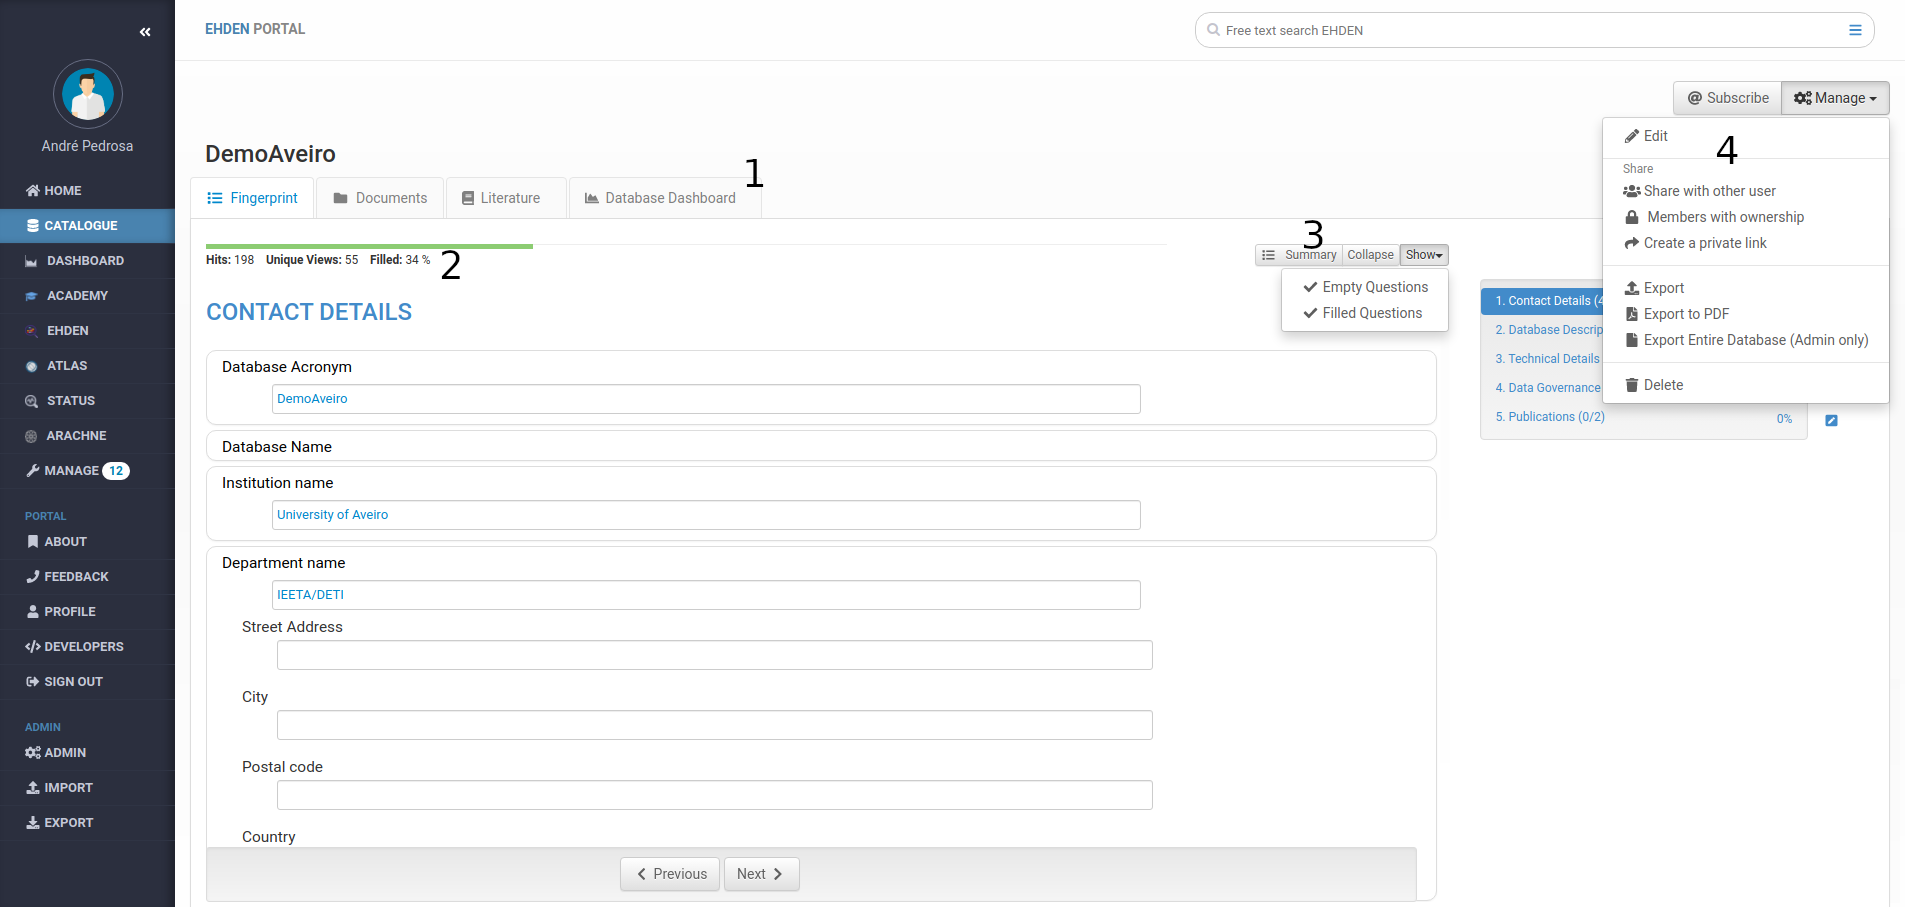
\includegraphics[width=\textwidth]{fingerprint-show-detailed}
    \caption{A detailed version user interface to view and analyze fingerprints}
    \label{fig:fingerprint-show-detailed}
\end{figure}

On the show view, if the user enters the detailed view (Figure \ref{fig:fingerprint-show-detailed}), the user is presented with a table with three columns where each row contains the question number, name and the answer given.
On this view, by hovering over an empty answer container the user can send a request to the database owner to answer the specific question.

\begin{figure}[h]
    \center
    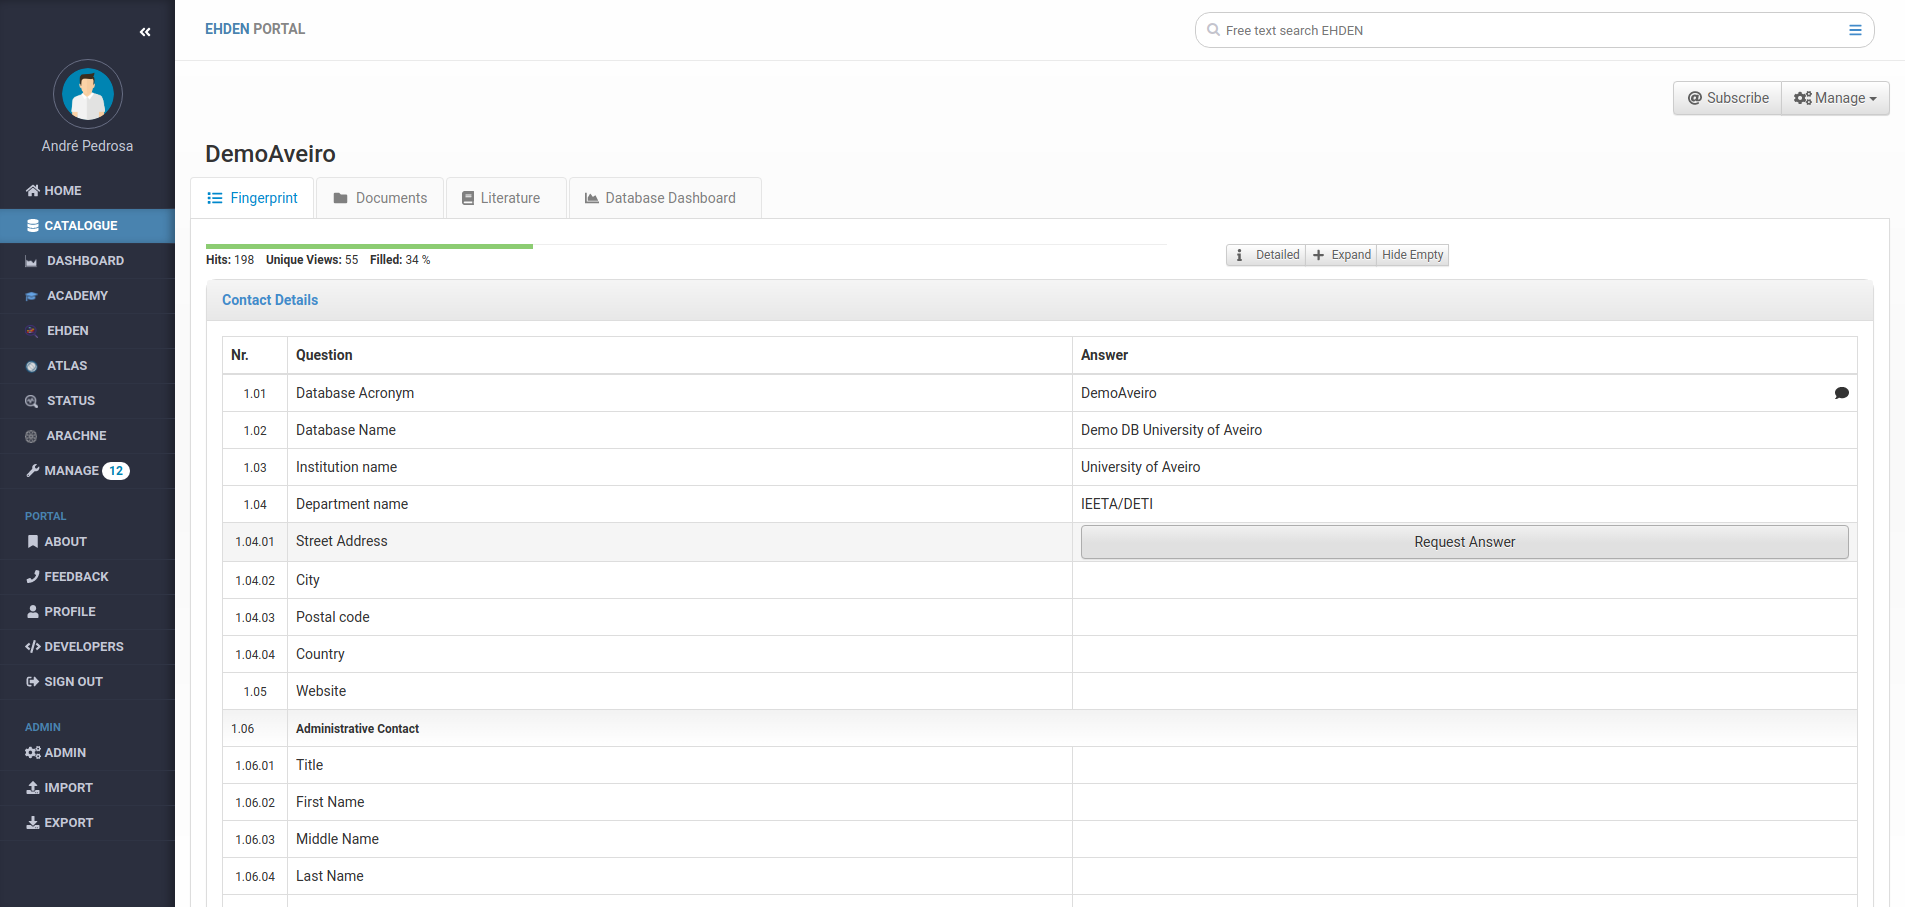
\includegraphics[width=\textwidth]{fingerprint-show-summary}
    \caption{A summary version user interface to view and analyze fingerprints}
    \label{fig:fingerprint-show-summary}
\end{figure}

This groups of view provide a valid workflow to perform \gls{crud} operation over the metadata related to a data source, however, present several flaws related to how the inputs are validated and how they are presented to the user.

First, the validation of the user input is done on the client-side through javascript code that runs after a user submits a question set form.
Subsequently, the data is sent to the backend through \gls{api} calls.
However, if one would use the \gls{api} directly to update metadata of the fingerprint, the validation could be skipped and invalid data could be stored on the database.
In some cases there might exist some validation code on the server-side, however, this brings the necessity to maintain two separate code files.

Second, there is no escaping procedure done to the user's input when it is fetched from the database which allows that \gls{xss} attacks can be easily performed and put users that consult a compromised fingerprint at risk.
As an example, on figure \ref{fig:montra-xss-create} on the Database Name field, I added a \textit{script} tag with code that shows a popup and also a valid database name after.
Once a user opens the fingerprint to check the data, the code will execute but the dummy name will render on the Database Name field.
This can be further exploited, where the user visiting the fingerprint will not notice that malicious code was executed.


\begin{figure}[h]
    \center
    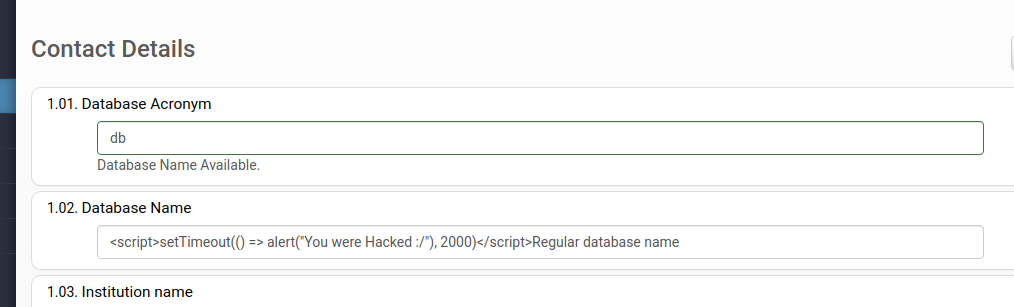
\includegraphics[width=0.75\textwidth]{montra-xss-create}
    \caption{Example of how an \gls{xss} attack could be done on MONTRA}
    \label{fig:montra-xss-create}
\end{figure}

\begin{figure}[h]
    \center
    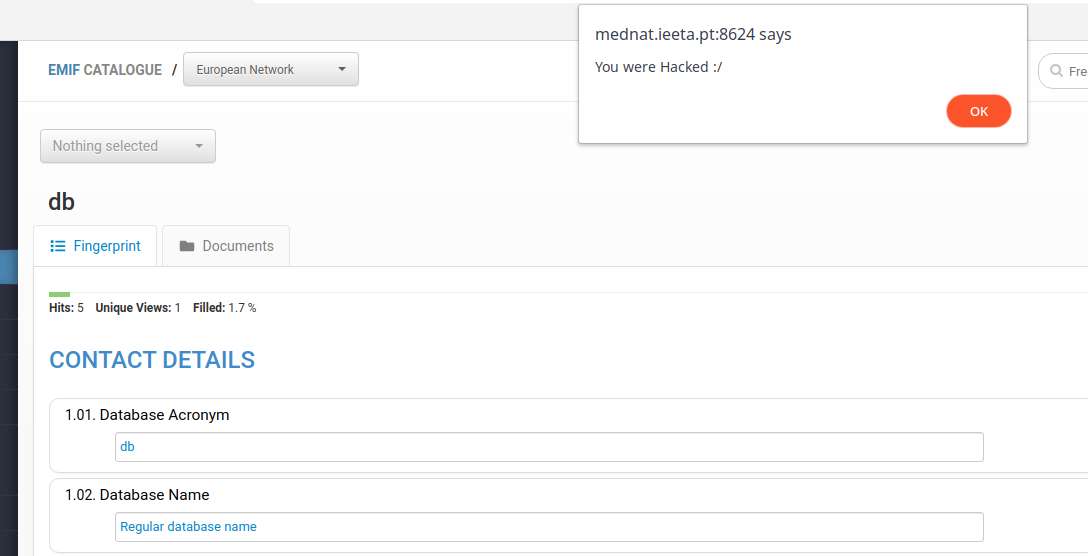
\includegraphics[width=0.75\textwidth]{montra-xss}
    \caption{Victim of a simple \gls{xss} attack}
    \label{fig:montra-xss}
\end{figure}

All these problems exist because such views were developed from scratch without using the provided features that Django has out of the box for form validation and security.
For client-side validation, Django takes advantage of HTML5 form validation features\footnote{\url{https://developer.mozilla.org/en-US/docs/Learn/Forms/Form_validation}}.
This allows imposing restrictions and validations on the user's input without writing any additional javascript code.

To show these features I wrote a simple HTML file with a simple form that expects a number under 100 and an email.

\begin{verbatim}
<html>
  <body>
    <form>
      <label for"num">Number:</label>
      <input id="num" type="number" max="100">

      <label for"mail">Email:</label>
      <input id="mail" type="email">

      <button type="submit">Submit</button>
    </form>
  </body>
</html>
\end{verbatim}

If I try to submit the form with invalid values, error messages are presented as shown in figure \ref{fig:html-form-validation}.

\begin{figure}[h]
    \center
    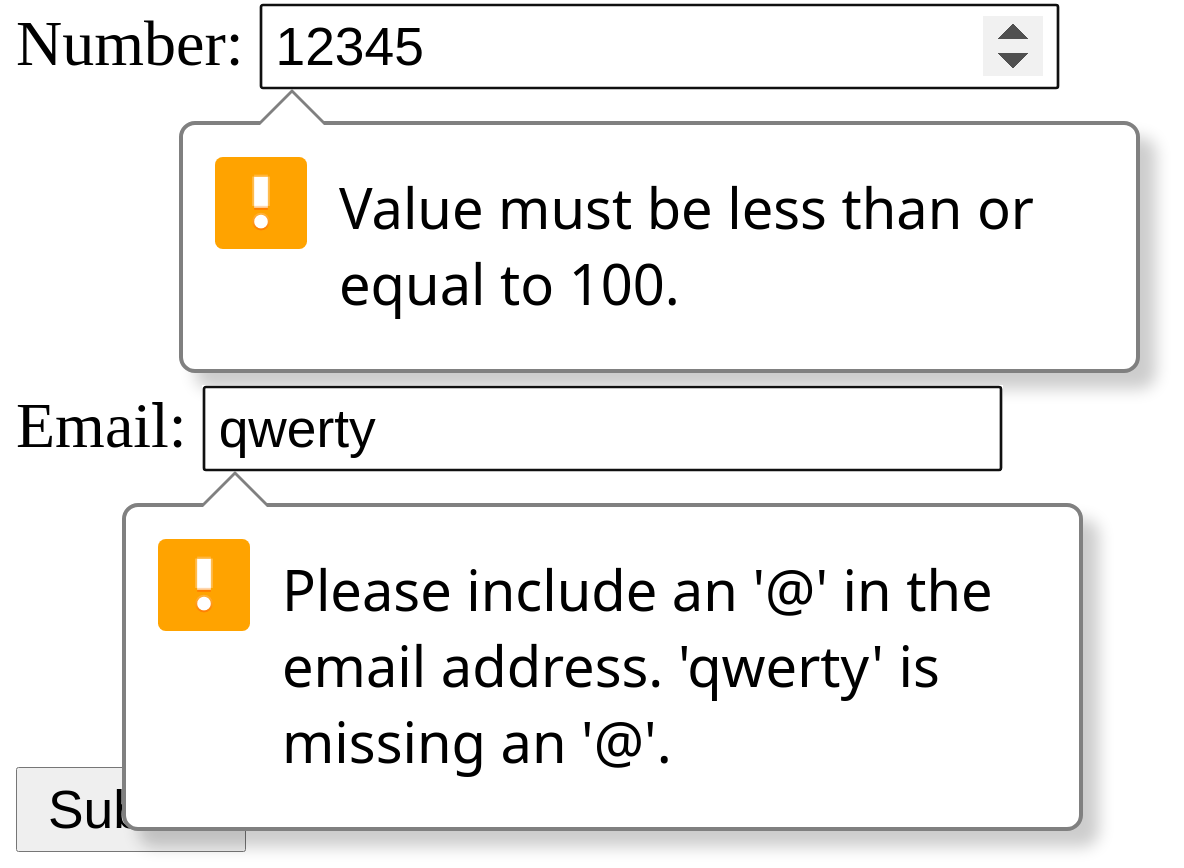
\includegraphics[width=.3\textwidth]{html-form-validation}
    \caption{Error messages that appear after submitting the form on a chromium based browser}
    \label{fig:html-form-validation}
\end{figure}

Additionally, if the data is sent directly through an \gls{api} call to the backend, Django forms framework ensures invalid data is rejected.
With this, when building a form in Django the developer only needs to specify what fields are present and their type and restrictions and Django will validate all this before data is stored on the database.

Finally, \gls{xss} attacks are prevented because Django escapes the values that were previously provided by users when filling the input tags, e.g. the character ``<'' is transformed in ``\&lt;'', avoiding the browser to interpret user's input as \gls{html} code.

\subsection*{API}

\begin{itemize}
    \item how submissions of fingerprint works
\end{itemize}

\subsection{Import Questionnaires - Excel}
\label{subsection:excel}

%\begin{itemize}
%    \item Como os vários conceitos anteriores são mapeados para o excel
%    \item Question Sets
%    \item Questions
%    \item Choices
%    \item ...
%\end{itemize}

As mentioned before, to define a skeleton of the metadata that describes a data source for a given community, a spreadsheet file has to be submitted.
There is already a template with some instructions and columns where a community manager only has to fill the necessary rows to then get the wanted result.

The column defined in the template are the following:
\begin{itemize}
    \item Type: the type of the specific row. Here are allows 3 different values:
        \begin{itemize}
            \item QuestionSet: allows dividing the questionnaire into several sections
            \item Question: a question specification
            \item Category: allows to create a group of questions inside a question set
        \end{itemize}
    \item Text/Question: label/name given to the item being defined
    \item Level/Number: use as a level for questions and categories and number otherwise. As level allows to create groups of questions inside a question set. As number defines the number, and subsequently the order, of the question sets.
    \item Data type: used only for rows of type Question, specifying the question type
    \item Value list: used to indicate extra information to build the question
    \item Help text/Description: a small text that will be displayed along with the item being defined
    \item Tooltip: Yes if the Help text/Description should be displayed as a tooltip or No otherwise
    \item Slug: internal identifier
    \item Dependencies: used to tell that a question or group of questions can only be answered if a specific choice of a choice-based question was selected
    %\item Stats: 
    %\item Comments Stats:
    %\item Disposition
    \item Include in Advanced Search: if the answers of the question can be used to search fingerprints
\end{itemize}

\subsection*{Question Groups}
From the previous list, question groups were mentioned both when the type column has the Category value and on the Level part of the Level/Number column.
The former is used to add a title with no question associated, resulting in what is presented in figure \ref{fig:question-group-category}.

\begin{figure}[h]
    \center
    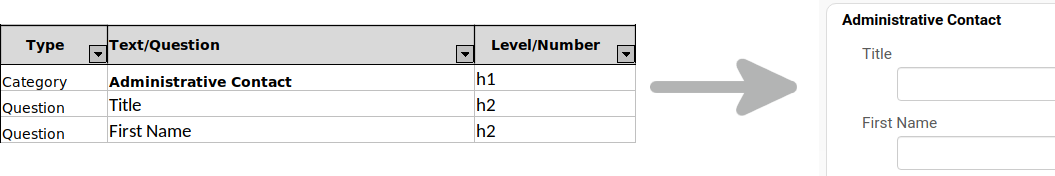
\includegraphics[width=\textwidth]{category}
    \caption{Create a group of questions with a title}
    \label{fig:question-group-category}
\end{figure}

On the latter, the text of the question in the most upper level is used as the title of the questions group, resulting in an output similar to the one in figure \ref{fig:question-group-levels}.

\begin{figure}[h]
    \center
    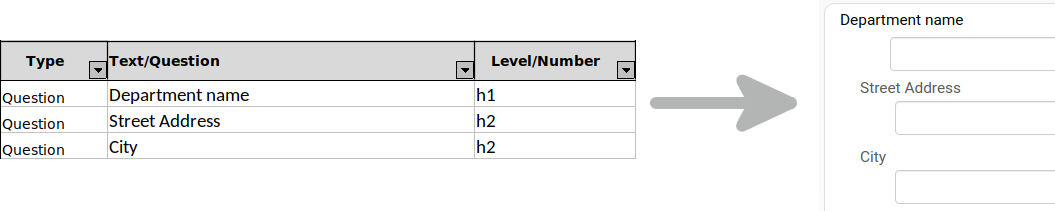
\includegraphics[width=\textwidth]{levels}
    \caption{Create a group of questions using a question's text as the title}
    \label{fig:question-group-levels}
\end{figure}

It's important to highlight that the category way to create question groups is not independent of levels.
If both a category row and a question are on the most upper level, MONTRA will render two separate collapsable containers, where the first one will be empty, as is shown in figure \ref{fig:question-group-category-wrong-levels}.

\begin{figure}[h]
    \center
    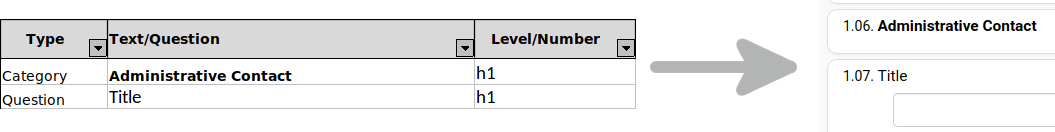
\includegraphics[width=\textwidth]{category-levels}
    \caption{Example to show that the category way to create question groups also depends on the values that are set on the level column}
    \label{fig:question-group-category-wrong-levels}
\end{figure}

\subsection*{Value list}

To avoid having a spreadsheet with several columns that will not be used for all types of rows, the value list column expects some extra information required for some types of questions.

\subsubsection*{Choices}

For choice-based questions, the value list column is used to define the possible choices and to add an extra text field associated with a given choice.
Choices are separated by a ``|'' character and the extra text field can be set by appending ``\{...\}'' after the target choice's text.

\begin{figure}[h]
    \center
    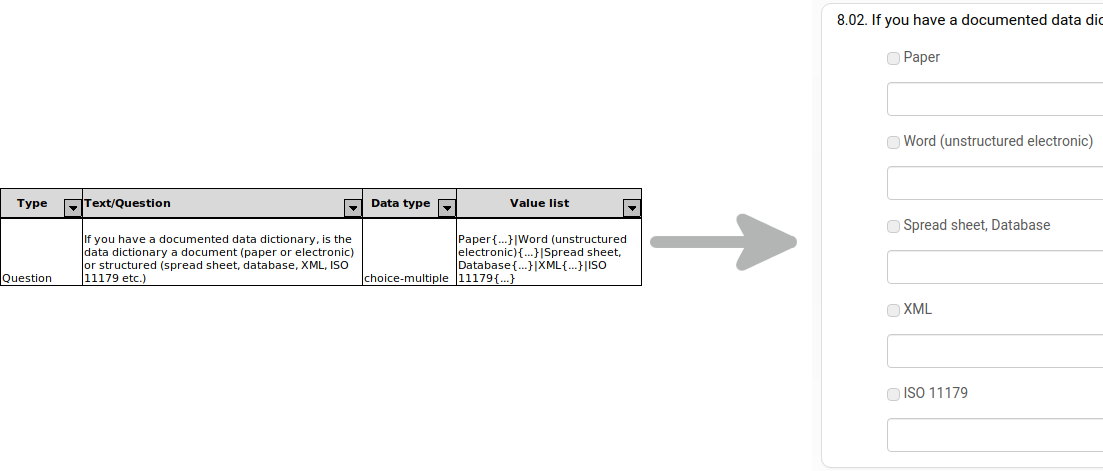
\includegraphics[width=\textwidth]{choice-freeforms}
    \caption{Multiple choice question with some extra text fields associated with the several choices}
\end{figure}

Although the framework allows the extensibility to have an additional text field, these don't support other types of input and also have no validation.
Also, if the number of choices is high and the text of them is long, there starts to exist some clutter on the spreadsheet.
With this, the person creating the spreadsheet will have problems perform edits and check if there is something wrong or missing.

To facilitate the job of who is filling the spreadsheet, some question types are shortcuts.
For example, the choice-yesnodontknow is a question of type choice with three possible options: Yes, No, Don't Know.
Choice variants with freeform on the name, besides the usual choices, always have an additional text field, associated with the question instead of a choice.

\subsubsection*{Open Multiple Composition}

Open multiple questions allow showing a history of a given value.
For that the simple version of the question is represented in a table of two columns: Date and the value, so no input is expected on the value list column.
The composition version of the question type allows having several values, instead of just one.
In a way, the simpler version can be used as a shortcut question type, since it can be reproduced with the composition variant.

To render this question type, a third-party widget called Tabulator\footnote{http://tabulator.info/} is being used.
The configuration of such widget, expects an array of \gls{json} objects, each specifying some configuration of each column.
To configure the open multiple composition question type, the value list column expects these \gls{json} objects, where the date column is implicit.
The MONTRA framework will then put the provided objects on the configuration array that the Tabulator widgets expects, adding the configuration for the date column.

\begin{figure}[h]
    \center
    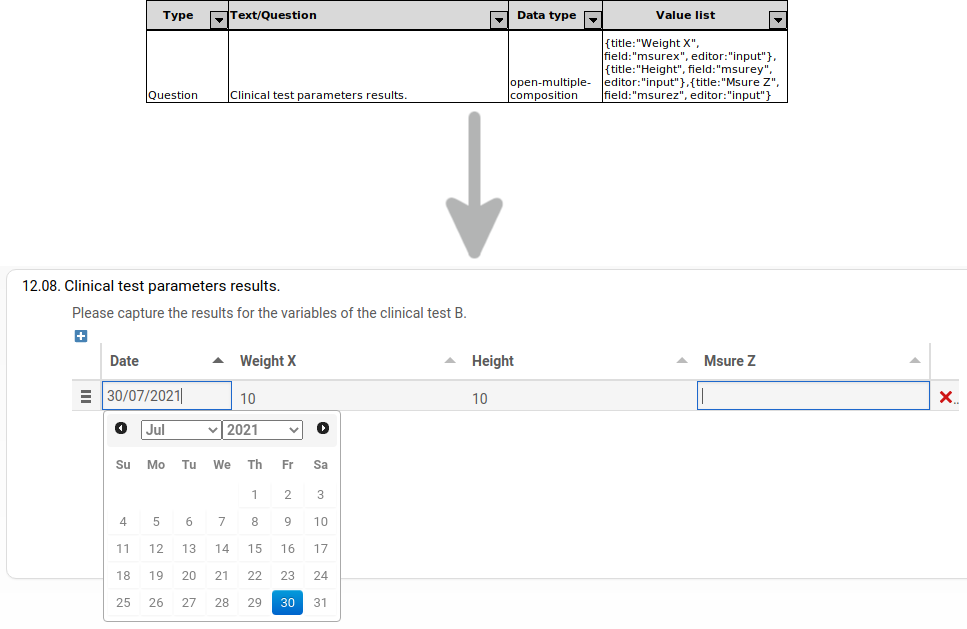
\includegraphics[width=\textwidth]{open-multiple}
    \caption{How an open-multiple-composition question type is specified on the spreadsheet and how it is rendered}
    \label{fig:open-multiple}
\end{figure}

\subsubsection*{Choice Tabular}

This type of question allows reusing the same choices across several answering items.
There are three variations of this questions types, where the difference between them is what and how is the information connected between answering items and choices.
There are two versions where the user can select one (single choice) or more (multiple-choice) choices for each answering item.
The other version allows the user to write text for each choice within each answering item.
The question type is rendered as a table where in the columns are displayed the several choices and on the rows the different answering items are presented.
Additionally, there is always a ``More'' choice column, where the user can insert any text information for a specific answering item since is displayed with a textarea \gls{html} element.

The value list column of a choice tabular question type expects a three-component value.
Each component is separated by the characters ``\textbackslash\textbackslash''.
Within each component, items are separated by the ``|'' character.
The components are the following:

\begin{itemize}
    \item choices (columns)
    \item answering items (rows)
    \item type of the information: available values are choice, multiple-choice and text
\end{itemize}

\begin{figure}[h]
    \center
    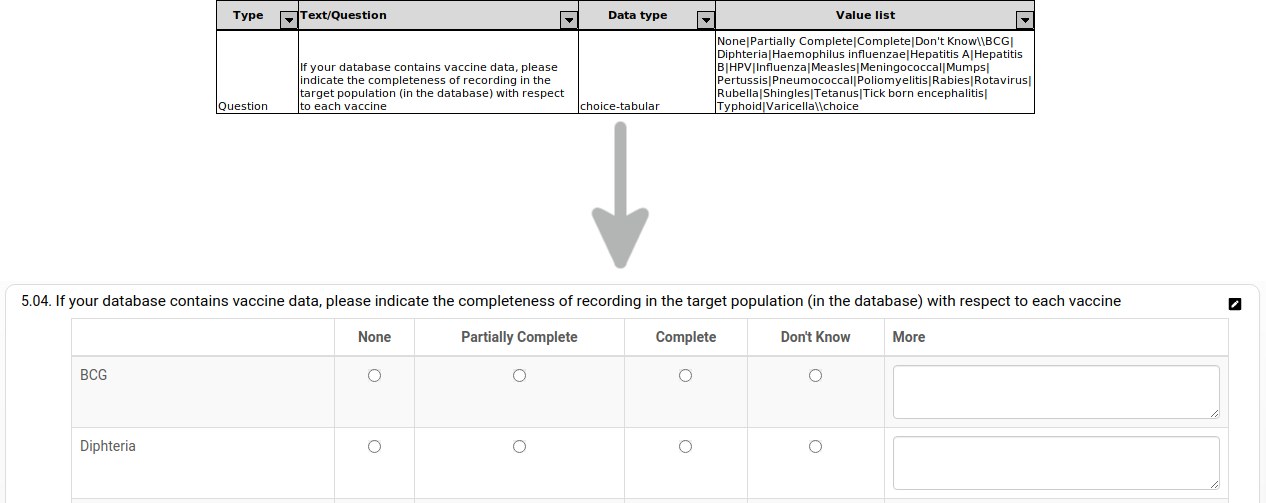
\includegraphics[width=\textwidth]{choice-tabular}
    \caption{How a tabular-choice question type is specified on the spreadsheet and how it is rendered}
    \label{fig:choice-tabular}
\end{figure}

Once again, we encounter the clutter problem, as shown in the spreadsheet section of figure \ref{fig:choice-tabular}, which hampers readability and update of the value list field.

\subsection*{Dependencies}

In several form applications, e.g. Google Forms, it is common to find situations where if a certain choice is selected, then other questions will show up.
E.g. If a user answers ``Yes'' to the Question ``Have you visited Aveiro?'', then other questions such as ``Would you recommend it to a friend?'' would appear.

MONTRA supports this kind of dependencies, which should be defined on the Dependencies column of the questionnaire spreadsheet.

\begin{figure}[h]
    \center
    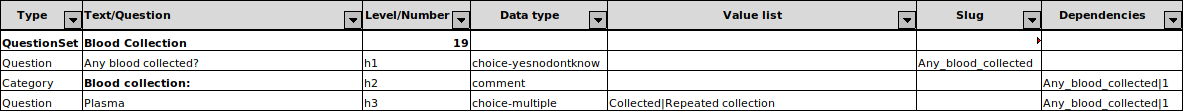
\includegraphics[width=\linewidth]{dependencies-excel}
    \caption{An example of both a question and a category that depend on the selected value for another question.}
    \label{fig:dependencies-excel}
\end{figure}

As shown in figure \ref{fig:dependencies-excel}, first you should indicate the slug of the question on which the specific question depends.
Then, separated by a ``|'' character, it must be specified which choice has to be selected for the dependency to be fulfilled, using its index, starting at 1.
On figure \ref{fig:dependencies-excel}, since a choice-yesnodontknow question type has three implicit choices, by having a dependency with the value ``Any\_blood\_collected|1'', both the \textit{Blood collection} category and the \textit{Plasma} question will only be displayed to the user once the choice \textit{Yes} of the \textit{Blood Collection} is selected.

\begin{figure}[h]
    \center
    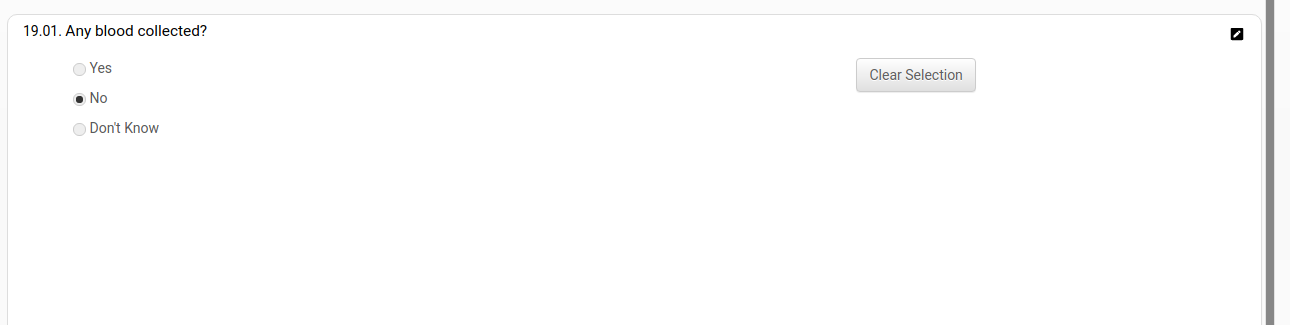
\includegraphics[width=0.75\linewidth]{dependencies-no}
    \caption{The questions with dependencies are not rendered if the specific choice is not selected}
    \label{fig:dependencies-no}
\end{figure}

\begin{figure}[h]
    \center
    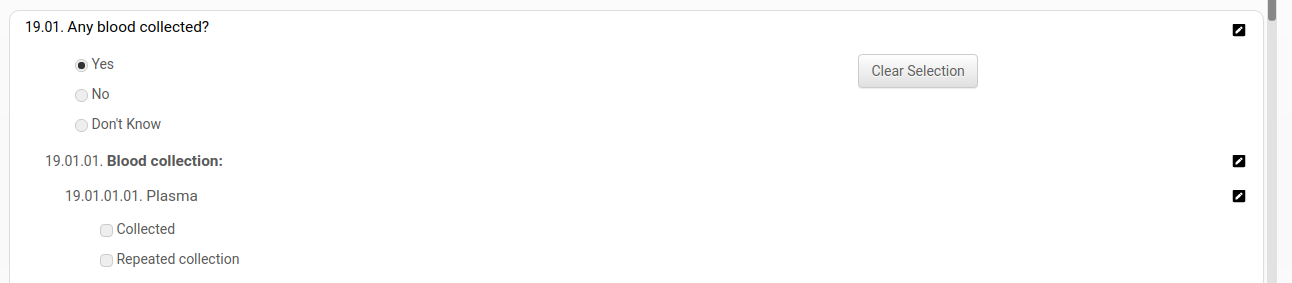
\includegraphics[width=0.75\linewidth]{dependencies-yes}
    \caption{Once the dependency of a specific question is meet it will be rendered}
    \label{fig:dependencies-yes}
\end{figure}

Besides such restrictions are imposed on the user when he visits the web page, if the API was used directly, such dependencies would not be checked, which would lead to unnecessary data be stored on the database since it won't be displayed to the user.

\subsection{Data Models}

%\begin{itemize}
%    \item Diagrama de classes
%    \item Principal intuito de cada class
%    \item answers (todos os tipos guardados em texto)
%\end{itemize}

This section will be presented how the previous concepts are mapped to database models.
Taking advantage of Django's \gls{orm} feature, MONTRA's data models are defined as python classes that extend Django's base Model class.
These Model classes belong to different applications, which are associated with distinct aspects of the platform.

In figure \ref{fig:old-models} is presented the class diagram of the classes that are related to features and/or concepts that were mentioned in previous sections.
Classes with the same color belong to the same Django application, dividing them into specific purposes.

\begin{figure}[h]
    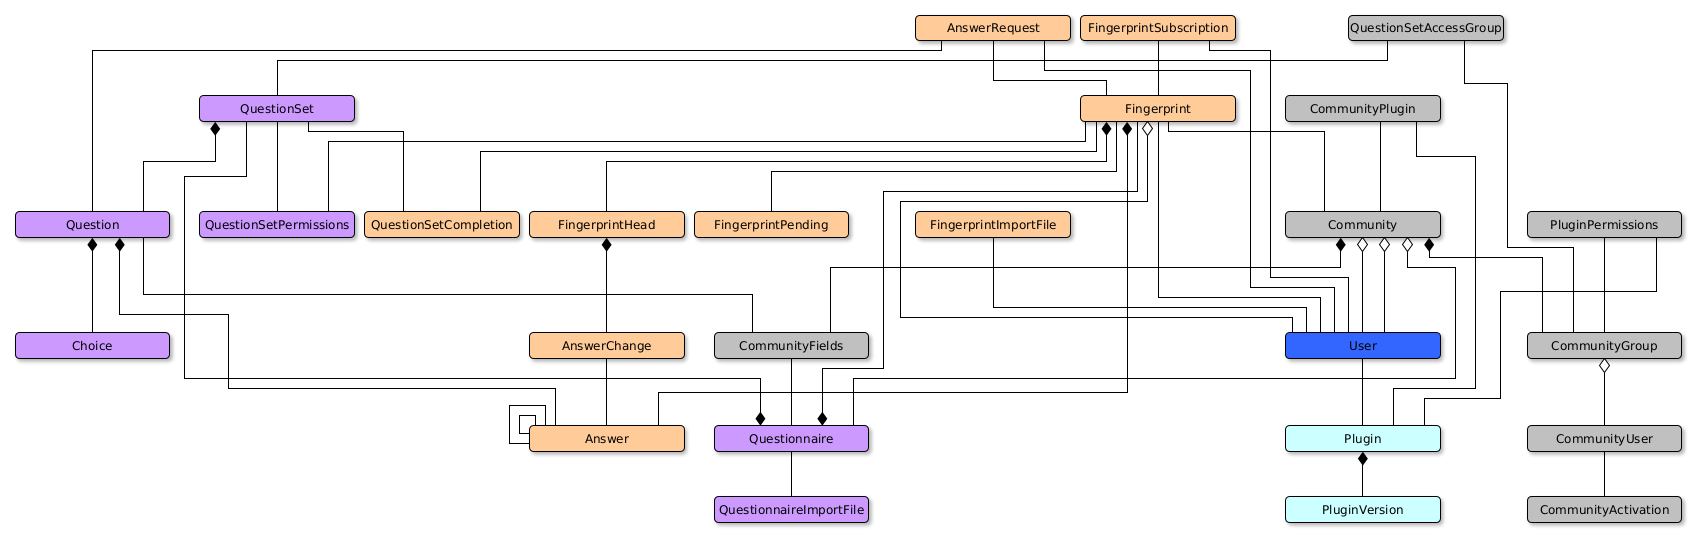
\includegraphics[width=\textwidth]{old-models}
    \caption{Class diagram of MONTRA's Model classes. Each color has a Django application associated. Gray: Community; Purple: Questionnaire; Orange: Fingerprint; Light Blue: Plugin; Blue: Django Auth. MONTRA's data model is much more complex, however, it is just presented the ones that impact the features and/or concepts mentioned previously.}
    \label{fig:old-models}
\end{figure}

\begin{itemize}
    \item Blue - Django's built-in authentication system\footnote{https://docs.djangoproject.com/en/1.11/ref/contrib/auth/}.
    \item Orange - Fingerprint application: Answers to questionnaires questions and other models associated with features that were mentioned on the fingerprint views section, such as AnswerRequest and FingerprintSubscription.
        MONTRA also keeps a record of all the states of a given Fingerprint.
        For that, it uses the FingerprintHead model, which maps to a set of AnswerChanges.
    \item Purple - Questionnaire application: Questionnaires structure information such as question sets, questions, and choices, and import spreadsheets logs. Additionally, associated with each fingerprint, contains a model with the allowed permissions on each question set.
    \item Light Blue - Developer application: Allows adding customizations to different MONTRA's installations through plugins.
    \item Gray - Community application: Community's groups, users and access permissions, fields to be presented on the fingerprint list page for each questionnaire and plugins.
\end{itemize}

Going into more detail on some models we can see some poor design decisions.

\begin{figure}[h]
    \center
    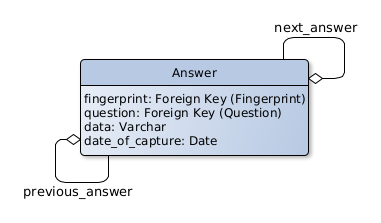
\includegraphics[width=.4\linewidth]{answer-model}
    \caption{Detailed information of the Answer model of the Fingerprint application}
    \label{fig:answer-model}
\end{figure}

Regarding fingerprint answers to a questionnaire, all the data is stored in the Answer model on the data field, which is a variable-length string field type.
Although this approach is much simpler in terms of data models, it leads to two problems:
\begin{enumerate}
    \item this is not the most optimized way to store all the data types.
        Some question types expect numeric values and other date values, which could use built-in field types of a relational BDMS.
    \item for complex question types which the answer contains several fields, before and after storing such data in the database, some processing has to be made to convert the data to the necessary format.
        One example of this is multiple choice questions, where the value of the several selected choice is joined in a single string to then be stored on the database.
        Every time the answer needs to be displayed to a user, it is necessary to split that string by its separator.
        For this situation instead of storing the choice's value, the models of the questionnaire application could be used as a foreign key.
\end{enumerate}

Related to MONTRA itself, when a user provides no data to a specific question, an empty string will still be sent for that question on the submission of the answers to a question set, which will create unnecessary records on the database.

\begin{figure}[h]
    \center
    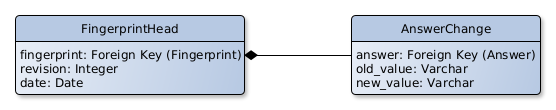
\includegraphics[width=.6\linewidth]{answer-changes-models}
    \caption{Models that store the changes to answers of fingerprint}
    \label{fig:answer-changes-models}
\end{figure}

As mentioned previously, MONTRA records the history of submissions for a specific fingerprint.
Each submission has an associated FingerprintHead record, which its name might have been inspired by the HEAD concept of Git\footnote{https://git-scm.com/}, a version control system.
For every FingerprintHead there is a set of answers that suffer changes which are then recorded on the AnswerChange model.
In this model, we can get the answers data duplicated three times since it is already stored on the Answer model and can also be stored again as text in both \textit{old\_value} and \textit{new\_value}.

\begin{figure}[h]
    \center
    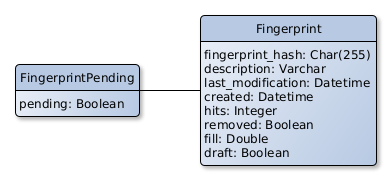
\includegraphics[width=.6\linewidth]{fingerprint-pending-models}
    \caption{The Model that stores the information telling if a fingerprint is waiting to be approved to be published}
    \label{fig:fingerprint-pending-model}
\end{figure}

As mentioned previously, a fingerprint is not immediately available to all regular users, since it first enters on a draft state.
To transit to the published state, a request needs to be made to the community owner.
Such requests are stored on the FingerprintPending table, where the pending value will be \textit{true}.
Once a request is rejected or accepted, the value of the pending value is changed to \textit{false}.

On the Fingerprint model, there is also a \textit{draft} value that indicates if the fingerprint is published or not.
Once a fingerprint is published, the value of the \textit{draft} will be true, and on the FingerprintPending table, the associated record will have the pending value at \textit{false}.
However, this value is not required to be stored on the database since after a fingerprint is published, the fingerprint will not be pending therefore, the associated FingerprintPending record could be deleted.

\begin{figure}[h]
    \center
    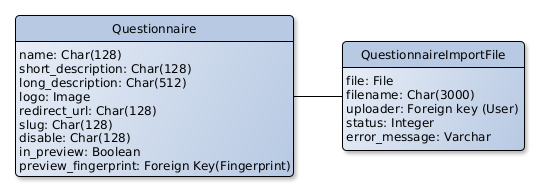
\includegraphics[width=.6\textwidth]{questionnaire-import-models}
    \caption{Questionnaire model and the model where questionnaire imports information is stored}
    \label{fig:questionnaire-import-models}
\end{figure}

Whenever a questionnaire is imported, a QuestionnaireImportFile record is created containing the information of the uploaded file and the user that uploaded it.
Also contains a status field to give some feedback to the user.
Associated with every import will also be created a Questionnaire record.
It contains an in\_preview variable that is set to \textit{true} whenever a questionnaire is in the import process.
If it fails to import, only the QuestionnaireImportFile record will be kept, which the status will change to \textit{Failed} and an error message will also be attached to the import record.

If the questionnaire is valid, the user will be redirected to a page where he can preview the result and can accept or reject it.
It is important to point out that for the preview process a new Fingerprint object is created so \gls{api} calls can be performed, to give a better preview experience to the user testing the questionnaire.
This preview fingerprint will be kept if the user decides to accept the questionnaire and deleted if it rejects.
Also, accepting will change questionnaire's in\_preview variable to \textit{false}.

Strangely on the Questionnaire model, the disable column uses a character type column instead of a boolean one since it expects only the value of ``False'' and ``True''.
If there are some user input errors, it could lead to unexpected behavior or internal server error.

\section{Refactoring}
\begin{itemize}
    \item o que necessita de, ou vai, ser alterado
\end{itemize}

\subsection{Data Models}
\begin{itemize}
    \item explicar escolha de apenas reformular apenas a apartir de determinado nivel
    \item explicar os novos modelos e de que maneiras resolvem problemas que existiam
    \item trade offs tidos em conta
    \item diagrama de classes com diferenças
    \item tipos de perguntas novos e deprecated
\end{itemize}

\subsection{Questionnaire}
\begin{itemize}
    \item UI changes
    \item consequencia da alteração do front end devido à alateração do backend
    \item passar toda a verificação para o backend, passando a usar a validação built in do Django
    \item tentar reutilizar os modulos existentes
\end{itemize}

\subsection{Excel}
\begin{itemize}
    \item mais concreto, e tem mais em conta o contexto em volta das questoes
    \item entanto é mais estenso
\end{itemize}
